%!TEX root = ../../report.tex
\chapter{Mapping of Dynamic Areas}
\label{mapping_of_dynamic_areas}
This chapter investigates possible methods for learning the dynamic properties of an area in order to improve localization and navigation. The dynamic learner module is shown in figure \ref{fig:dynamic_learner_overview} in relation to the rest of the dynamic mapping system. The dynamic learner receives the static map snapshots and uses these as the basis for learning the dynamics.  


\begin{figure}[htbp]
	\centering
	\includegraphics[scale=1]{chapters/mapping_of_dynamic_areas/figures/dynamic_overview.eps}
	\caption{The static mapping in the dynamic mapping system}
	\label{fig:dynamic_learner_overview}
\end{figure}

\section{Learning Dynamics of Occupancy Grid}
\label{sec:learning_dynamics_of_env}

\subsection{Previous work}
Learning the dynamics of an environment is a subject with ongoing research.
An early system for mapping the dynamics of the environment in a occupancy grid was the Temporal Occupancy Grid (TOG) proposed by Arbucle et al. \cite{Arbuckle2002}. The TOG system maintains several occupancy grids based on different time scales. This requires storing the observations for the time the longest TOG spans. It can be difficult to determine the time scales needed to estimate the differently and changing dynamic behaviors in the environment.

Biber and Duckett \cite{Biber2005} proposes a method for mapping environment dynamics with maps that represent observations taking over different periods of time. The method is here denoted as Temporal Sample Map (TSM). The maps are updated by incorporating measurements using different recency weighted running average functions. These functions are estimated by removing random observations. The highly dynamic obstacles are considered as outliers and up to $50\%$ of them are removed by using the median measurement.

An avenue of thought that has received quite a lot of attention is the representation and learning of a Markov process based grid. A Markov Chain based grid was introduced by Sarinnen et al. \cite{Saarinen2012} called Independent Markov Chain Occupancy grid map (IMAC). This method represents each cell as a Markov process that can be in either of the states; free or occupied. 

\begin{figure}[tbph]
	\centering
	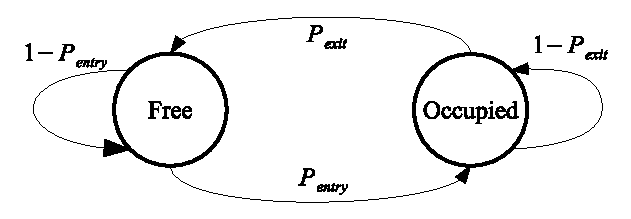
\includegraphics[width=0.7\linewidth]{chapters/mapping_of_dynamic_areas/figures/markow_occupancy_model}
	\caption{Markow chain for occupancy states borrowed from \cite{Saarinen2012}}
	\label{fig:markow_occupancy_model}
\end{figure}

The transitions is modeled as Poisson processes and the rate parameters is estimated as Gamma distributions. This gives in total four variables for each cell, which are used to interpret the type of dynamic for the cell. 

Another method for learning the map dynamics using Hidden Markov Models (HMM) is described by Meyer-Delius et al. \cite{Meyer-Delius2012}. This method uses the same possible states as the IMAC, but as it is a HMM the states are not directly observable thus it is possible to incorporate sensor uncertainty. In order to learn the parameters of the model two methods are used; an offline and an online approach. The offline approach requires storing all observations and then iteratively learn the parameters using the expectation-maximization algorithm. The online version of the parameter learning algorithm, developed by Mongillo and Deneve \cite{Mongillo2008} eliminates the need for storing the whole observation set. Instead only 16 values has to be stored for each cell and the iterative learning can be done online. The online method is capable of handling changing dynamics by using a forget factor. 

A different approach to mapping the dynamics is the Frequency Map Enhancement (FREMEN) proposed by Krajník et al. \cite{Krajnik2014}. This method models the dynamics of each cell by its primary frequency components. 
For prediction of future state the frequencies are reconstructed to a signal, which determines the predicted cell value. 
These uses a limited and constant number of parameters per cell. However, the method also requires the storage of time spans where the prediction went wrong in order to determine when a new model is needed. This significantly increases the memory requirements of the method.

With the reconstructed signal it is possible to predict infinitely long out in the future if it object moves with that frequency. 
This is not the case for Markow processes where the predicted probability for being in a state stabilizes on a constant, after many state changes.
There are also disadvantages with the method.
The most prominent comes from the fact, that it is impossible to recover a signal with a frequency lower than the Rayleigh-frequency of $1/T$, where $T$ is the period. 
This demands for storing measurements for the time period in which objects appears, disappears and appears again. This period can everything from hours for vehicles to days or weeks for stocked product parts. 
It might be possible to degrease the amount of stored information by only storing the average taken over periods, but then it is impossible reconstruct objects moving faster than the period which the average is taken. 

The characteristics of the six methods to improve occupancy grid mapping by learning the dynamics of the environment are outlined in table \ref{tab:learners_characteristics}.

\begin{table}[htbp]
    \centering
    \caption{Characteristics of methods to learn dynamics in occupancy grids.}
    \label{tab:learners_characteristics}
    \begin{tabular}{p{2.6cm} | p{1.6cm} | p{4.cm} | p{2.6cm} | p{1.6cm}}
        \toprule
        \textbf{Name} & \textbf{Memory} & \textbf{Dynamic representation} & \textbf{Learning method} & \textbf{Handles dynamics} \\
        \rowcolor[gray]{0.925}
        TOG & High & Time averaged OG & Online batch & Yes \\
        TSM & High & Time  averaged OG & Random sample replacement  & Yes\\
        \rowcolor[gray]{0.925}
        IMAC & Low & Markov parameters & Online iterative & Yes \\
        HMM - Offline & High & Markov parameters & Offline batch  & No \\
        \rowcolor[gray]{0.925} 
        HMM - Online & Low & Markov parameters & Online iterative & Yes \\
        FREMEN & Medium & Frequency components & Online batch & Yes\\
        \bottomrule
    \end{tabular}
\end{table}

\subsection{Methods ability to learn Markow Processes}
The described methods that models dynamic with Markow processes are compared with a simple simulation where a grid cell are occupied by a dynamic obstacle. 
Whether the cell is occupied or free is controlled by a Markow process with $0.9$ probability for entering and $0.2$ probability for exiting the cell. 
The process is observed by an one dimensional range sensor, which can measure too short with a probability of $0.16$, in which case the online-HMM are propagated one step without adding new information and the IMAC is left unchanged.
There is an equal probability for the sensor measuring a range too far, which results in a reading of an empty cell independently of the cell's state. 
Figure \ref{fig:markow_learning} shows that IMAC is unable to converge to the correct state transition probabilities, where as the HMM-online method that incorporate the uncertainties in measurements slowly converges toward them.
The state transitions estimated by IMAC are so far from the actual parameters that they are almost useless for prediction. 
The number of measurements needed for HMM-online to converge is however very large.
Considering that the simulation is setup so that the object has a considerable possibility of moving between each measurement, it will be very time consuming to learn the transition probabilities for obstacles moving at days between.

\begin{figure}[htbp]
    \centering
    \begin{subfigure}[t]{0.45\textwidth}
        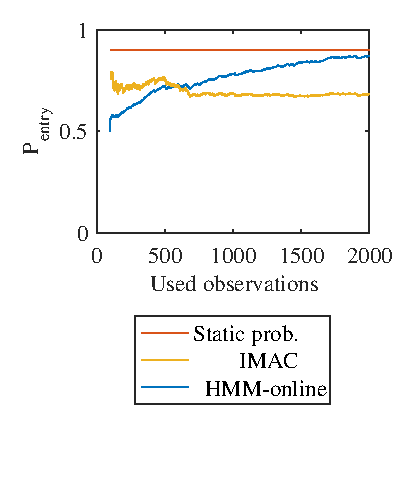
\includegraphics[width=1.0\textwidth]{chapters/mapping_of_dynamic_areas/figures/markow_learn_1d_entry}	
        %\caption{}
        %\label{fig:markow_learn_1d_entry}
    \end{subfigure}
    \begin{subfigure}[t]{0.45\textwidth}
        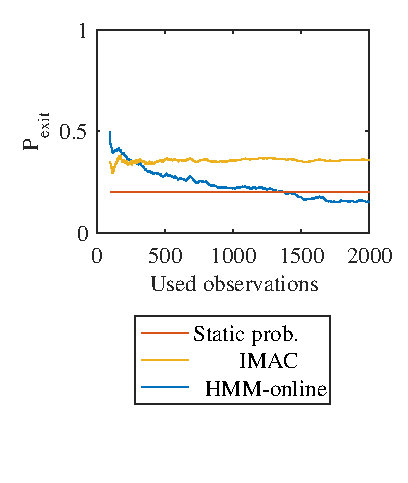
\includegraphics[width=1.0\textwidth]{chapters/mapping_of_dynamic_areas/figures/markow_learn_1d_exit}
        %\caption{}
        %\label{fig:markow_learn_1d_exit}
    \end{subfigure}
    \caption{Learned state transition probabilities compared to the simulated Markow process.}
    \label{fig:markow_learning}
\end{figure}

\section{FreMEn - Predicting future occupancy}
\label{sec:fremen}
The  Frequency Map Enhancement (FreMEn) method models the dynamics of each cell by its primary frequency components. It has successfully been applied to improve mobile robots ability to perform feature-based localization \cite{online_fremen} and topological navigation \cite{fentanes2015}. Here Krajník et al. argues for approximating the appearance and disappearance of obstacles with multiple periodic sinus signals, since people often moves them as part of daily routines. As discussed in section \ref{sec:characteristics_in_industrial_environments} this might also be the case in the industrial environments in focus here. Resent work in \cite{life_long_exploration}, shows how the often violated assumption in FFT about a fixed sampling rate is met by incrementally adding sparse and irregular observations. Where the approach usually uses the number of frequency components(m) that minimizes the difference between predicted states and measurements, it is chosen to use the typical order m=2 \cite{life_long_exploration} for all cells. This will probably decrease the prediction performance, but enables online updates without having to store observations for evaluation.

The online variant of the approach updates the parameters shown in equation \ref{eq:fremen_time} for each new measurement $s(t)$. 
The average occupancy probability $\alpha_0$ models the $0Hz$ signal and is updated with a new measurement online. 
The number of measurements n is incremented. There is one of the complex numbers $\gamma_k$ and $\beta_k$ for each $\omega_k=1/T_k$ . 
$T$ is calculated with equation \ref{eq:fremen_update} for each frequency, where N is the 20 used frequency components and epsilon is the smallest period time, which is one minute here. 
The values of consecutive $T_k$ is close for large values of $k$, which is advantageous if most of the obstacles moves with a period close to $\epsilon$.

\begin{equation}
    T_k = \frac{N \epsilon}{k+1}
    \label{eq:fremen_time}
\end{equation}

The real and imaginary part of $\gamma_k$ and $\beta_k$ are updated as the running average. $\gamma_k$ is the part of the signal with the frequency $2 \pi \omega_k$ and $\beta_k$ is the part of this signal which are modeled by the $0Hz$ component of the signal.

\begin{eqnarray}
&\alpha_0 = \frac{1}{n+1}(n \alpha_0 + s(t)) \nonumber \\ 
&\gamma_k = \frac{1}{n+1}(n \gamma_k + s(t) e^{-j \omega_k t}) \forall \omega_k \in \Omega  \\
&\beta = \frac{1}{n+1}(n \beta_k + \alpha_0 e^{-j \omega_k t}) \forall \omega_k \in \Omega \nonumber \\
&n = n + 1 \nonumber
\label{eq:fremen_update}
\end{eqnarray}

When predicting the state of a cell at time $t$ the signal components are calculated with equation \ref{eq:fremen_freq_component}.

\begin{equation}
    \alpha_k = \gamma_k - \beta_k \forall \omega_k \in \Omega
    \label{eq:fremen_freq_component}
\end{equation}

Then $ \Omega $ is ordered based $ | \alpha_k | $ to enable calculation of equation \ref{eq:fremen_predict} using only the $m$ most prominent frequency components. As previously described, we use two frequency components ($ m=2 $) for each cell.

\begin{equation}
p(t) = \zeta \left( \alpha_0 \sum_{k=1}^{m} |\alpha_k| cos(\omega_k t + arg(\alpha_k))  \right)
\label{eq:fremen_predict}
\end{equation}

The function $\zeta$ clamps the expected probability to a value between zero and one. The $arg$-function returns the angle of the complex number with respect to the x-axis.
The occupancy state at time $t$ is predicted as occupied if $p(t)$ is above $0.5$ and as free otherwise.

\begin{figure}[htbp]
\centering
\includegraphics[width=0.4\linewidth]{chapters/mapping_of_dynamic_areas/figures/simulated_environment}
\caption{Screen shot of Stage simulator showing a MIR 100 robot navigating around obstacles which appears and disappears at fixed intervals.}
\label{fig:simulated_environment}
\end{figure}

The methods ability to predict future occupancy states are evaluated in a Stage simulation where many boxes moves in and out at various and fixed, intervals. 
The robot continuously navigates from the lower left corner that are partly surrounded by walls to the top right corner, while the red and green boxes moves around.
The measurements from the simulated LIDAR are incorporated in a temporary local map using the reduced ideal inverse sensor model update method described in section \ref{sec:reduced_ideal_sensor_model}. 
The update values for the sensor model is reduced to incorporate uncertainties in localization.
For every fifth second a global map of FreMEn cells are updated with \ref{eq:fremen_update} where $s(t)$ is the probability for occupancy in the local map. 
The local map is then cleared and the process continues.

\begin{figure}[htbp]
    \centering
    \begin{subfigure}[t]{0.49\textwidth}
        \includegraphics[width=1.0\textwidth]{chapters/mapping_of_dynamic_areas/figures/fremen_ideal_simulation}	
        \caption{Predicted map without noise.}
        \label{fig:fremen_ideal_sim}
    \end{subfigure}
    \begin{subfigure}[t]{0.49\textwidth}
        \includegraphics[width=1.0\textwidth]{chapters/mapping_of_dynamic_areas/figures/fremen_with_decay_last}
        \caption{Predicted map with realistic sensor and localization noise.}
        \label{fig:fremen_sim_with_noise}
    \end{subfigure}
    \caption{Robot navigating in the map predicted with FreMEn where the the green dots marks ends of LIDAR readings.}
\end{figure}

To evaluate the predictive strength of FreMEn it is used to predict the appearance of obstacles each time a new measurement is added from the local map. 
Figure \ref{fig:fremen_ideal_sim} shows how FreMEn correctly predicts the appearance of many of the obstacles when the robots exact position is used to incorporate exact LIDAR measurements. 
Figure \ref{fig:fremen_avg_miss_with_noise} shows a more realistic simulation with Gaussian noise on LIDAR measurements with a standard deviation of one centimeter and localization using AMCL with a static map representation.
Here some of the obstacles are predicted to have moved while they in fact are still present, as shown in the middle to the right in figure \ref{fig:fremen_avg_miss_with_noise}.

FreMEn's lack of ability to predict future measured obstacles is also apparent in the average correctly predicted observations of obstacles. 
This is shown in figure \ref{fig:fremen_avg_correct_predictions} where the good prediction percent on $74.0\%$ drops to $46.9\%$ with the addition of noise.
From the experiment without noise it is concluded that the learned periodic appearance of obstacles in a grid with FreMEn is useful for predictions.
In the presence of noise the signals within the cells becomes more complicated, and the measurements used for comparison is not always correct.
This, combined with the fact that obstacles placed by humans probably will not move in and out of grid cells so consistently as in this simulation, leads us to believe that the implemented method is not useful for online update of the occupancy grid map used by AMCL.
It might however be possible to alter the method, or combine it with others, to take advantage of the methods ability to predict presence of obstacles many hours after the last observation.
The predicted maps can improve the validness of global paths planned by the robot, but with the rather poor prediction percentage many paths have to be re-planned during navigation. 

\begin{figure}[htbp]
    \centering
    \begin{subfigure}[t]{0.49\textwidth}
        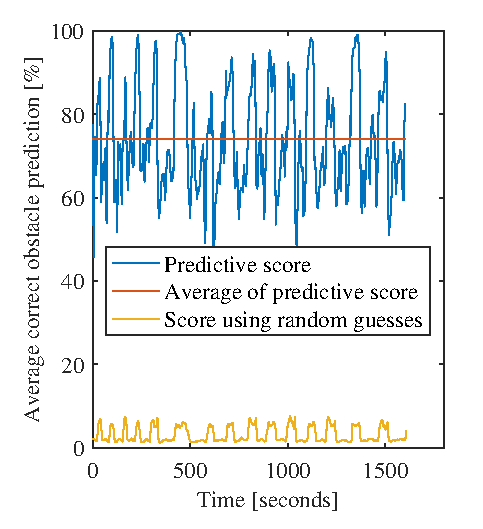
\includegraphics[width=1.0\textwidth]{chapters/mapping_of_dynamic_areas/figures/fremen_avg_miss_no_noise}	
        \caption{Prediction score without noise.}
        \label{fig:fremen_avg_miss_no_noise}
    \end{subfigure}
    \begin{subfigure}[t]{0.49\textwidth}
        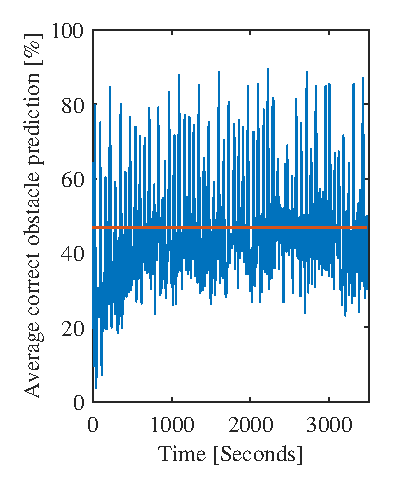
\includegraphics[width=1.0\textwidth]{chapters/mapping_of_dynamic_areas/figures/fremen_avg_miss_with_noise}
        \caption{Prediction score with noise.}
        \label{fig:fremen_avg_miss_with_noise}
    \end{subfigure}
    \caption{Prediction scores for FreMEn defined as the average number of matches between measured and predicted obstacles.}
    \label{fig:fremen_avg_correct_predictions}
\end{figure}

%!TEX root = ../../report.tex
\section{ Probabilistic Input  Markov Chain}
\label{sec:pmac}

\subsection{Developing on independent Markov chains}
The IMAC method considers an observation to be either occupied or free. In the system setup used in this project, however, the input is the probability that a cell is occupied. To use IMAC it is necessary to determine the state of the observation with one or two thresholds. The simplest choice is placing a threshold at $0.5$ rendering everything above as an occupied observation and everything below a free. This approach will make no distinction between an observation of $0.501$ and $0.999$, which both will be considered occupied and contribute equally in the learning process. This is not desirable as the latter measurement contains immensely more information than the former. 
Equating all measurements on the basis that they fall on the same side of a threshold reduces the advantage of taking position and sensor noise into consideration. An example could be a cell observed at a great distance and quite large uncertainty and then later very close by with high confidence in the reading. These two entries into the IMAC learner would carry the same weight. If for instance a reading resulted in a $0.99$ occupancy probability and a following reading produced a $0.49$ occupancy probability, the simple threshold method would register it as an occupied followed by a free and thus adding an event. In reality there is very little evidence for this event happening and if the subsequent reading would again produce a $0.99$ occupancy probability this would introduce even more dynamics disregarding that the evidence is very unsubstantiated. 

Therefore a method of incorporating the uncertainty of the observations and carrying them into the learner is desired. As IMAC is a fast learner of Markov transition probabilities when the observations are very certain, the incorporation of the uncertainties should not hinder that. 

The requirements for the incorporation of the uncertainties are:
\begin{itemize}
	\item Perform as IMAC on perfect input
	\item Avoid low confidence observations counting as much as high confidence
	\item Avoid biasing towards neither static or dynamic
\end{itemize}

The method devised to accomplish the integration of uncertainties is denoted probability input Markov chain (PMAC). As opposed to IMAC the PMAC uses a score rather than a count of a state and event. The state score is calculated as  \(2\cdot|0.5-p_{occ}|\) for the active state which is determined by whether \(p_{occ} > 0.5\) or not. This ensures that if the reading is certain, ie. either 0 or 1 the update will be similar to that of IMAC, and as uncertainty increases the score linearly decreases. The event score is calculated based on how certain the previous state was and how certain the current state is. In order to avoid biasing towards dynamic the maximum, based on the certainty of the previous state, is the average of the consecutive observations in that state. As the average cannot exceed 1 this ensures that in perfect certainty the behavior is equal to that of IMAC. The maximum limit based on the current state is the sum of scores in the current state.

\begin{equation}
IMAC: \lambda = \frac{\#event_{count}}{\#state_{obs}}
\end{equation}

\begin{equation}
PMAC: \lambda = \frac{\Sigma event_{score}}{\Sigma state_{score}}
\label{eq:pmac_lambda}
\end{equation}

\begin{equation}
state_{score}=2 \cdot |0.5-p_{occ}| 
\end{equation}

\begin{equation}
event_{score}=min(\hat{\mu}_{state_{score}}(i-1),state_{score}(i))
\end{equation}

Both the state and event scores behave as IMAC counters when the certainty is perfect, thus fulfilling the first requirement. The second requirement is achieved by the state score scaling with the occupancy probability distance from $0.5$, and the event score basing its value on the state score. Basing the state score on the distance from $0.5$ helps to avoid skewing the result towards static. Another possible scoring could be the probability for occupied and free respectively: 

\begin{equation}
score_{occ} = p_{occ}
\end{equation}
\begin{equation}
score_{free} = 1-p_{occ}
\end{equation}

As the active state is determined by a threshold of $0.5$, this scoring system would always be at least $0.5$, skewing the results. The chosen score better incorporates $0.5$ denoting unknown, thus producing a score of $0$. 

In order to avoid biasing towards dynamic the average of the previous state scores is used. If, instead, the sum had been used, a series of low confidence observations could skew the result. As the state score can be considered $\hat{\mu} \cdot n_{obs}$ the event score will be balanced when using as a maximum value. For instance $5$ observation with an occupancy probability of $0.6$ would each give a score of $0.2$, and the sum would consequently be $1$. Using the sum,  would be $1/1$  thus skewing it towards dynamics. Using the average, the event score is balanced to the state score and produces a more correct value of $0.2/1$. The correctness of this result is evident from the fact that simply counting events and states with IMAC also results in a probability on $\lambda = 1/5$. Hence the correct dynamics is estimated with PMAC and the parameters are only updated according to the confidence in the used observations.

\subsection{PMAC in action - an example}
Figure \ref{fig:state_scores_explained} shows an example of some observation, their occupied probabilities $p_{occ}$ and the subsequent state score. On the score plot the average of sequential observation in the same state are shown as green lines. This sets a maximum limit on the size of the subsequent event score. To demonstrate the workings of PMAC these observations are used as input to the PMAC learner in the following. 

\begin{figure} [htbp]
    \centering
    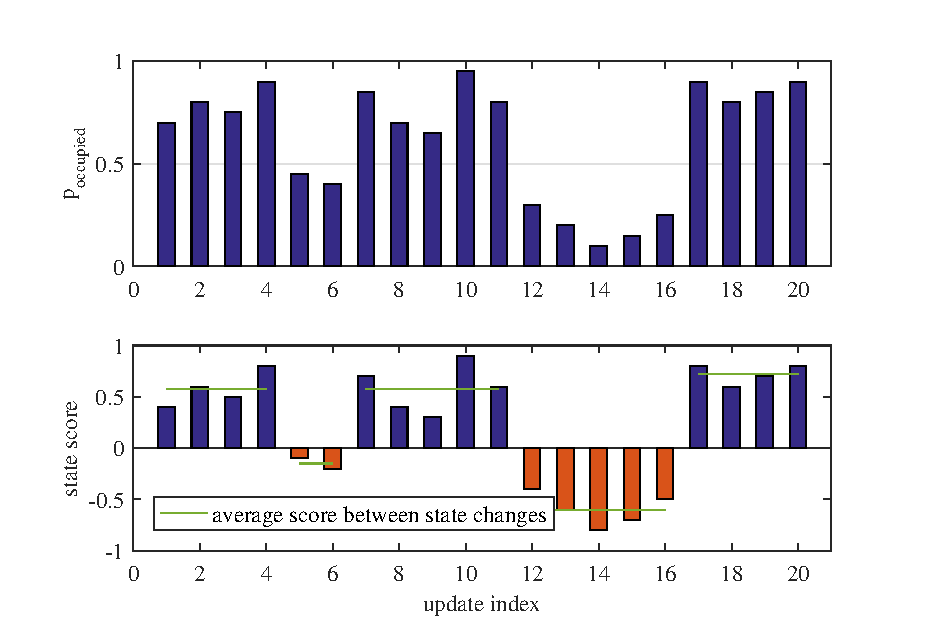
\includegraphics[scale=1]{chapters/mapping_of_dynamic_areas/figures/state_scores_explained}
    \caption{Artificial example of occupancy probabilities used to learn dynamics.}
    \label{fig:state_scores_explained}
\end{figure}

From the state scores in figure \ref{fig:state_scores_explained} it is seen that from index 0 to 11, the situation starts as occupied with quite confident readings. Then $2$ more uncertain reading showing free occurs before confident readings of occupied are again received. The effect of this on the exit is shown in figure \ref{fig:pmac_exit_explained}. The sum of occupied scores increases steadily from index $0$ to $11$, while the event sum increases a comparatively small amount. However it is clearly visible on the exit  value as it is the first observations and both sums are initialized to the smallest possible non-zero value. This initialization is chosen in order to avoid dividing by $0$ and minimizing the effect of the initialization on the result. The effects of this initialization is clearly visible in figure \ref{fig:pmac_entry_explained}, that shows the scores and values for the entry. The entry value is $1$, as the initial values causes, but as soon as input is received their effect is suppressed.

\begin{figure}[htbp]
\centering
\includegraphics[scale=1]{chapters/mapping_of_dynamic_areas/figures/pmac_exit_explained}
\caption{Evolution of parameters used to estimate dynamics with the data shown in figure \ref{fig:state_scores_explained}.}
\label{fig:pmac_exit_explained}
\end{figure}

The observations from index $7$ to $20$ constitutes more certain changes in the state and thus carry more information which can be seen in the sums of especially the free score and entry event score. 

\begin{figure}[htbp]
    \centering
    \includegraphics[scale=1]{chapters/mapping_of_dynamic_areas/figures/pmac_entry_explained}
    \caption{Evolution of parameters used to estimate dynamics with the data shown in figure \ref{fig:state_scores_explained}.}
    \label{fig:pmac_entry_explained}
\end{figure}

\todo{Write about improved pmac handling noise problem}

\begin{figure}[htbp]
\centering
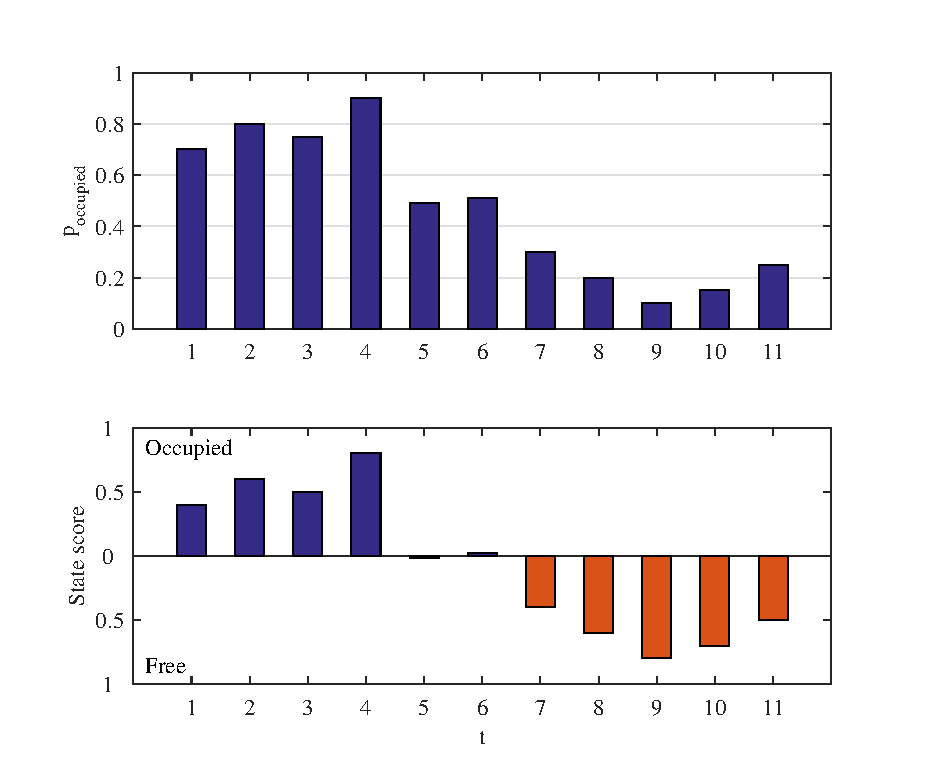
\includegraphics[scale=1]{chapters/mapping_of_dynamic_areas/figures/pmac_noise_problem_case}
\caption{}
\label{fig:pmac_noise_problem_case}
\end{figure}


\begin{figure}[htbp]
    \centering
    \includegraphics[scale=1]{chapters/mapping_of_dynamic_areas/figures/visualization_of_advantage_long_term_average}
    \caption{}
    \label{fig:visualization_of_advantage_long_term_average}
\end{figure}

%INSERT ENTRY FIGURE



Disucussion on underlying Markov model -> Accuracy, Realism

\subsection{Initializing the dynamic map}
As the dynamic map is the result of a learning process it will not contain any information from the onset. 
This might be a problem if the localization and navigation systems are relying on the results to perform their tasks.
To handle this, but also to guide the dynamic map it is possible to initialize the PMAC parameters. 
This could be done by what has previously been learned by the PMAC or by a static map.
The initialization value of the PMAC parameters should be set according to the desired output, considering the interpretation, and  the confidence in the initial map.
If the confidence is high in the obstacles of the initializing map, giving the cells in the dynamic map a strong initialization helps ensure that small errors will have less effect. 
The same principles go for the free areas but it is likely might become obstructed at some point so initializing them too heavily might reduce the usefulness of the dynamic learner.
Three different types of initialization is available from a static map; free, occupied and unknown.
Each type can have different user-defined initialization values in order to accommodate various use-cases.  

%!TEX root = ../../report.tex
\section{Summary}


\begin{figure}[htbp]
	\centering
	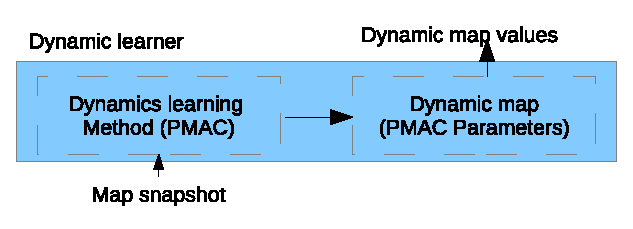
\includegraphics[scale=1]{chapters/mapping_of_dynamic_areas/figures/dynamic_detail.eps}
	\caption{The static mapping in the dynamic mapping system}
	\label{fig:dynamic_learner_detail}
\end{figure}



